\subsection{Spiking Neural Networkの構成}

Spiking Neural Network (SNN) は前述したニューロンにおけるパルス信号を介した情報処理を模倣したニューラルネットワークである\cite{generalsnn}.
そのため, 通常のArtificial Neural Network (ANN) と比較して, より生物的妥当性が高いモデルと考えられている.
SNNはパルス状の電気信号を, スパイクと呼ばれる0か1の値を持つ信号として扱う.
さらに, スパイクが時間軸に沿って並べられたものをスパイク列と呼び, SNNはこのスパイク列をニューロン間で伝達することで, ニューロンの時間的なダイナミクスを模倣し情報処理を行う.

SNNの第$l$層における入出力の流れを\figref{fig:snn:inoutflow}に示す.
まず, SNNへ入力されたスパイク$\bm{o}^{t, l-1}$は\eqrefc{eq:input_spike}によって重み付けされシナプス電流$\bm{i}^{t,l}$へ変換される.

\begin{equation}
    \bm{i}^{t, l} = \bm{W}^l\bm{o}^{t, l-1} + \bm{b}^l
    \label{eq:input_spike}
\end{equation}
ここで, $t$はその時刻を表し, $\bm{W}^l, \bm{b}^l$はそれぞれ第$l$層のニューラルネットワークの重みとバイアスを表す.

次に, 第$l$層のSNNの内部状態$\bm{v}^{t, l}$は, 神経細胞活動の数理モデルによって更新される.
本研究では, 数理モデルとしてLeaky Integrate-and-Fire (LIF) モデル\eqrefc{eq:lif}を用いる.
LIFモデルとは, 入力シナプス電流を, 神経細胞の内部状態があるしきい値に達するまで時間的に積分するモデルである.

\begin{equation}
    {\tau}\frac{d\bm{v}^l}{dt}=-\left(\bm{v}^l\left({t-1}\right)-v_{rest}\right)+r\bm{i}^{t, l}
    \label{eq:lif}
\end{equation}
ここで, $\tau$は神経細胞の時定数, $v_{rest}$は内部状態の初期状態, $r$は神経細胞の膜抵抗である.

最後に, 内部状態$\bm{v}^{t, l}$が一定の閾値$v_{th}$を超えたときに出力スパイク$\bm{o}^{t, l}$が1となって出力される (\eqrefc{eq:outputSpike}).
また, 閾値を超えた内部状態は初期状態へとリセットされる (\eqrefc{eq:outputSpike2}).

\begin{equation}
    \begin{split}
      \bm{o}^{t, l}&=g\left(\bm{v}^{t, l}\right)\\
    where\\
    g\left(x\right)&=\left\{
      \begin{alignedat}{2}
        1 &\:\left(x{\geq}v_{th}\right)\\
        0 &\:\left(x{<}v_{th}\right)
      \end{alignedat}
    \right. 
    \end{split} \label{eq:outputSpike}
  \end{equation}

  \begin{equation}
    \begin{split}
      \bm{v}^{t, l}&=h\left(\bm{v}^{t, l}\right)\\
    where\\
    h\left(x\right)&=\left\{
      \begin{alignedat}{2}
        &v_{rset} &\:\left(x{\geq}v_{th}\right)\\
        &x &\:\left(x{<}v_{th}\right)
      \end{alignedat}
    \right. 
    \end{split} \label{eq:outputSpike2}
  \end{equation}


\begin{figure}[htb]
    \centering
    % \includesvg[width=0.9\textwidth, inkscapelatex=false]{Static/chap2_sec1_snn}
    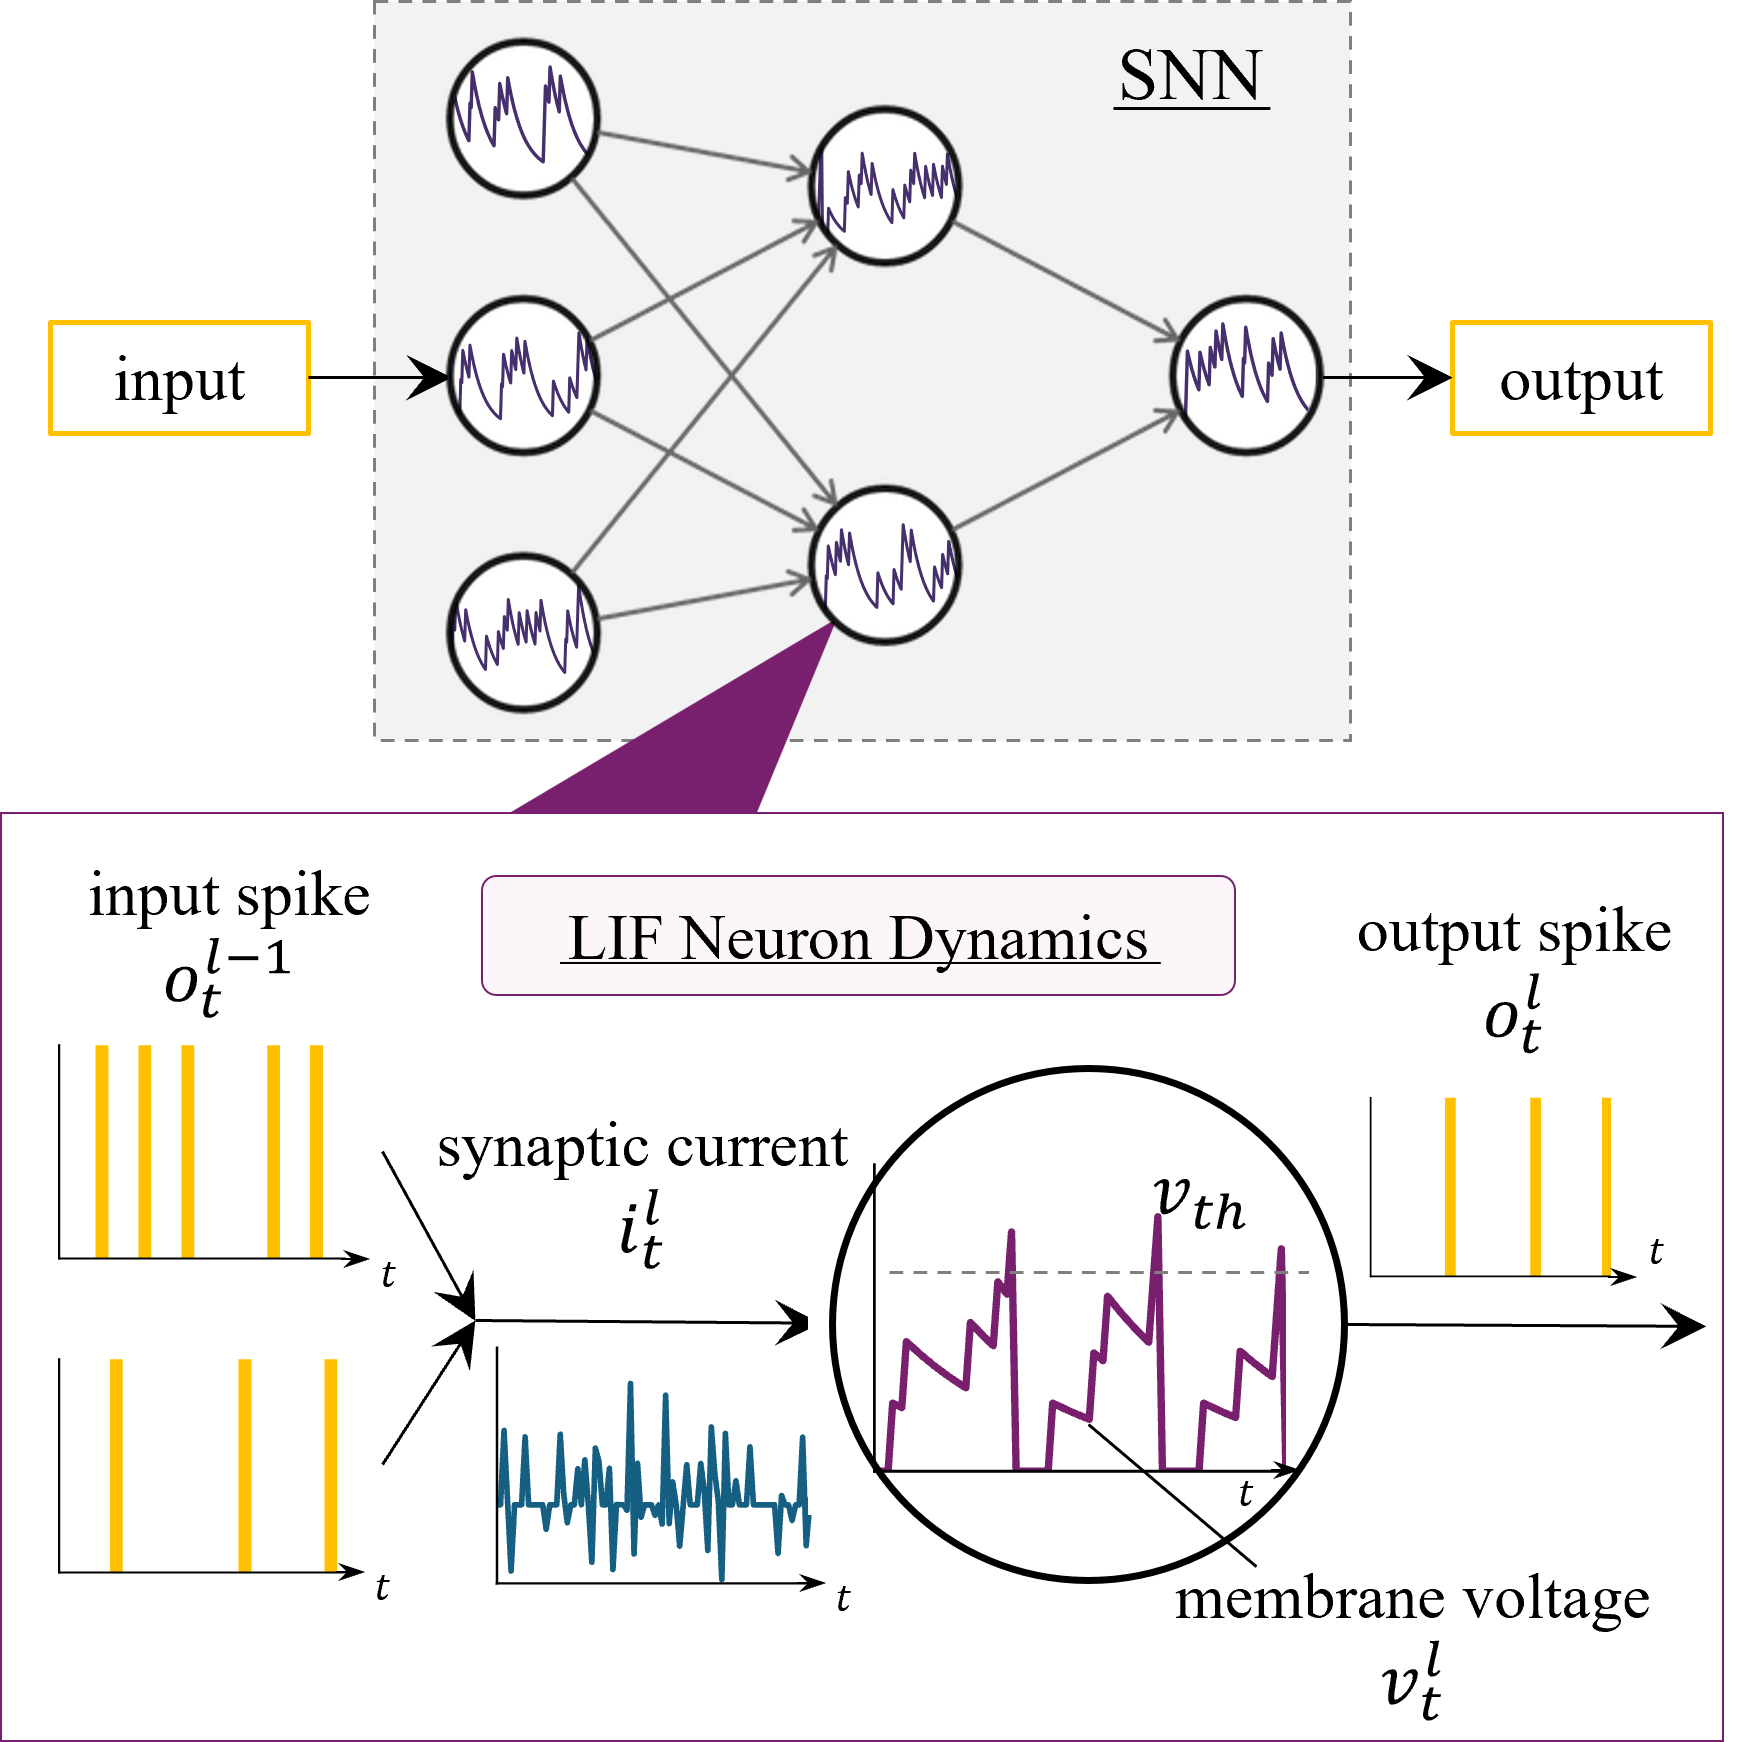
\includegraphics[width=0.75\textwidth]{Static/chap2_sec1_snn.png}
    \caption{SNNの入出力の流れ}
    \label{fig:snn:inoutflow}
\end{figure}
